\documentclass[11pt,]{article}
\usepackage[left=1in,top=1in,right=1in,bottom=1in]{geometry}
\newcommand*{\authorfont}{\fontfamily{phv}\selectfont}
\usepackage[]{mathpazo}


  \usepackage[T1]{fontenc}
  \usepackage[utf8]{inputenc}



\usepackage{abstract}
\renewcommand{\abstractname}{}    % clear the title
\renewcommand{\absnamepos}{empty} % originally center

\renewenvironment{abstract}
 {{%
    \setlength{\leftmargin}{0mm}
    \setlength{\rightmargin}{\leftmargin}%
  }%
  \relax}
 {\endlist}

\makeatletter
\def\@maketitle{%
  \newpage
%  \null
%  \vskip 2em%
%  \begin{center}%
  \let \footnote \thanks
    {\fontsize{18}{20}\selectfont\raggedright  \setlength{\parindent}{0pt} \@title \par}%
}
%\fi
\makeatother




\setcounter{secnumdepth}{3}


\usepackage{graphicx,grffile}
\makeatletter
\def\maxwidth{\ifdim\Gin@nat@width>\linewidth\linewidth\else\Gin@nat@width\fi}
\def\maxheight{\ifdim\Gin@nat@height>\textheight\textheight\else\Gin@nat@height\fi}
\makeatother
% Scale images if necessary, so that they will not overflow the page
% margins by default, and it is still possible to overwrite the defaults
% using explicit options in \includegraphics[width, height, ...]{}
\setkeys{Gin}{width=\maxwidth,height=\maxheight,keepaspectratio}

\title{Título\\
Subtítulo\\
Subtítulo  }



\author{\Large Cinthia Amalia Vandepool Candelario\vspace{0.05in} \newline\normalsize\emph{Estudiante de Geografia, Universidad Autónoma de Santo Domingo (UASD)}  }


\date{}

\usepackage{titlesec}

\titleformat*{\section}{\normalsize\bfseries}
\titleformat*{\subsection}{\normalsize\itshape}
\titleformat*{\subsubsection}{\normalsize\itshape}
\titleformat*{\paragraph}{\normalsize\itshape}
\titleformat*{\subparagraph}{\normalsize\itshape}

\titlespacing{\section}
{0pt}{36pt}{0pt}
\titlespacing{\subsection}
{0pt}{36pt}{0pt}
\titlespacing{\subsubsection}
{0pt}{36pt}{0pt}





\newtheorem{hypothesis}{Hypothesis}
\usepackage{setspace}

\makeatletter
\@ifpackageloaded{hyperref}{}{%
\ifxetex
  \PassOptionsToPackage{hyphens}{url}\usepackage[setpagesize=false, % page size defined by xetex
              unicode=false, % unicode breaks when used with xetex
              xetex]{hyperref}
\else
  \PassOptionsToPackage{hyphens}{url}\usepackage[unicode=true]{hyperref}
\fi
}

\@ifpackageloaded{color}{
    \PassOptionsToPackage{usenames,dvipsnames}{color}
}{%
    \usepackage[usenames,dvipsnames]{color}
}
\makeatother
\hypersetup{breaklinks=true,
            bookmarks=true,
            pdfauthor={Cinthia Amalia Vandepool Candelario (Estudiante de Geografia, Universidad Autónoma de Santo Domingo (UASD))},
             pdfkeywords = {morfometría fluvial, modelo digital de elevación, red de drenaje, razón
de bifurcación},  
            pdftitle={Título\\
Subtítulo\\
Subtítulo},
            colorlinks=true,
            citecolor=blue,
            urlcolor=blue,
            linkcolor=magenta,
            pdfborder={0 0 0}}
\urlstyle{same}  % don't use monospace font for urls

% set default figure placement to htbp
\makeatletter
\def\fps@figure{htbp}
\makeatother

\usepackage{pdflscape} \newcommand{\blandscape}{\begin{landscape}}
\newcommand{\elandscape}{\end{landscape}}


% add tightlist ----------
\providecommand{\tightlist}{%
\setlength{\itemsep}{0pt}\setlength{\parskip}{0pt}}

\begin{document}
	
% \pagenumbering{arabic}% resets `page` counter to 1 
%
% \maketitle

{% \usefont{T1}{pnc}{m}{n}
\setlength{\parindent}{0pt}
\thispagestyle{plain}
{\fontsize{18}{20}\selectfont\raggedright 
\maketitle  % title \par  

}

{
   \vskip 13.5pt\relax \normalsize\fontsize{11}{12} 
\textbf{\authorfont Cinthia Amalia Vandepool Candelario} \hskip 15pt \emph{\small Estudiante de Geografia, Universidad Autónoma de Santo Domingo (UASD)}   

}

}








\begin{abstract}

    \hbox{\vrule height .2pt width 39.14pc}

    \vskip 8.5pt % \small 

\noindent Resumen del manuscrito


\vskip 8.5pt \noindent \emph{Keywords}: morfometría fluvial, modelo digital de elevación, red de drenaje, razón
de bifurcación \par

    \hbox{\vrule height .2pt width 39.14pc}



\end{abstract}


\vskip 6.5pt


\noindent  \section{Introducción}\label{introducciuxf3n}

A lo largo del último siglo se ha reducido la dificultad para realizar
analisis espaciales gracias a los novedosos avances tecnologicos, el
desarrollo de los Sistemas de Información Geografica (SIG) ha
simplificado el arduo trabajo que suponia llevar acabo analisis
espaciales, aunque a pesar de todas las herramientas \{\} disponibles la
República Dominicana aún está pasos por detras de muchos paises en
especial en lo relacionado a los analisis morfometricos de cuencas
hidrograficas, situación lamentable ya que la isla posee innumerables
cursos de agua permitiéndole ocupar un lugar privilegiado en este siglo,
ya que cada día, más país sufren por la escases de agua dulce potable.

La cuenca hidrográfica a analizar en esta investigación es la
Microcuenca Caña, perteneciente a la Subcuenca del Rio Macasía, ubicada
en el extremo suroeste de la República Dominicana, dicho análisis se
realizará basandonos en datos preexistentes a partir de un \emph{modelo
digital de elevación (DEM)}, el cual es un modelo simbólico, de
estructura numérica y digital que pretende representar la distribución
espacial de la elevación del terreno, siendo la altura una variable
escalar que se distribuye en un espacio bi-dimensional (Burgos \&
Salcedo (2014)).

La morfometría fluvial se encarga de analizar los parámetros
morfometricos de una cuenca hidrográfica, tales como, la red de drenaje,
la pendiente, la forma, el orden de la red y demás aspectos fisicos.(@)
Entendiendo que la cuenca hidrográfica es ese sistema o unidad
geográfica e hidrológica formada por un rio principal y todo el
territorio entre el origen del rio y su desembocadura, interactúando en
este espacio diversos factores bióticos y abióticos.

El aspecto general de una cuenca se entiende como la forma en la que se
distribuyen los cursos de agua, esta forma depende princiapalmente de la
gravedad y la pendiente. Diversos autores ha establecido metodos tanto
cualitativos como cuantitativos para determinar la forma de la cuenca,
ademas de que han establecido clasificaciones para denominar a las
cuencas con formas similares (ej: Dendrítica); Cuando nos referimos a la
red de drenaje de una cuenca estamos refiriendonos a la relacion entre
la logitud total de los cursos fluviales de todos los ordenes y el área
de la cuenca, esta variable nos permitira establecer las caracteristicas
litologicas del área de estudio (Elorza (2008)).

Además, debemos tomar en cuenta, que el orden de red de los cursos de
una cuenca indica el grado de ramificacion de la red fluvial; existen
distintos metodos para jerarquizar los cursos de una red pero los dos
más conocidos y utilizados son el metodo de Strahler (1952) y el de
Horton (1945), gracias a esta jerarquización se puede entender mejor el
comportamiento del sistema de drenaje de la cuenca, ademas de que se
puede obtener la razon de bifurcación descrita por Horton como la
relación entre el número de cursos de un orden y número de cursos de
orden más alto, esta propiedad es condicionada por la forma que presenta
la cuenca (Elorza (2008) Lux Cardona (2016) Ibañez Asensio, Moreno
Ramón, \& Gisbert Blanquer (2011)).

Gutierrez-Elorza (2008), sostiene que el perfil longitudinal de una rio
es la linea obtenida a partir de las diferecias de alturas desde su
afloramiento hasta desembocar en otro cuerpo de agua, este perfil es
cóncavoe aunque no todos los rios lo presentan de manera clara debido a
afloramientos de rocas duras, actividad tectonica reciente o debido a
cambios subitos del caudal (Elorza (2008)). A partir del Indice de
Concavidad observaremos si la cuenca en cuestión presenta realmente un
perfil concavo y en caso de no serlo trataremos de identificar las
posibles causas.

Debido a la escases de datos sobre las caracteristicas morfometricas de
las cuencas de la República Dominicana esta investigación pretende
aportar datos reales sobre la morfometria de la microcuenca caña con el
objetivo de que puedan ser usados para realizar futuros estudios sobre
el comportamiento hidrologico de la microcuenca ante eventos climaticos
y sus posibles incidencias en las poblaciones asentadas en su margen.

\section{Metodología}\label{metodologuxeda}

\subsection{Área de Estudio}\label{uxe1rea-de-estudio}

El rio caña nace en la vertiente Norte de la Sierra de Neiba
aproximadamente a unos 1,400 metros sobre el nivel del mar. Respecto a
su division politico-administrativa la Microcuenca del Rio Caña abarca
los municipios de El Cercado y Las Matas de Farfan en la provincia de
San Juan y las comunidades de El Llano, Juan Santiago y Hondo Valle de
la provinica de Elias Piña. Geograficamente se localiza entre las
coordenadas 18\(^\circ\) 56' 25.32" N y 18\(^\circ\) 37' 39.64" N
latitud norte y 71\(^\circ\) 27' 18.45" W y 71\(^\circ\) 44' 03.63" W
longitud oeste Ministerio de Medio ambiente y Recursos naturales (2016).

\begin{figure}
\centering
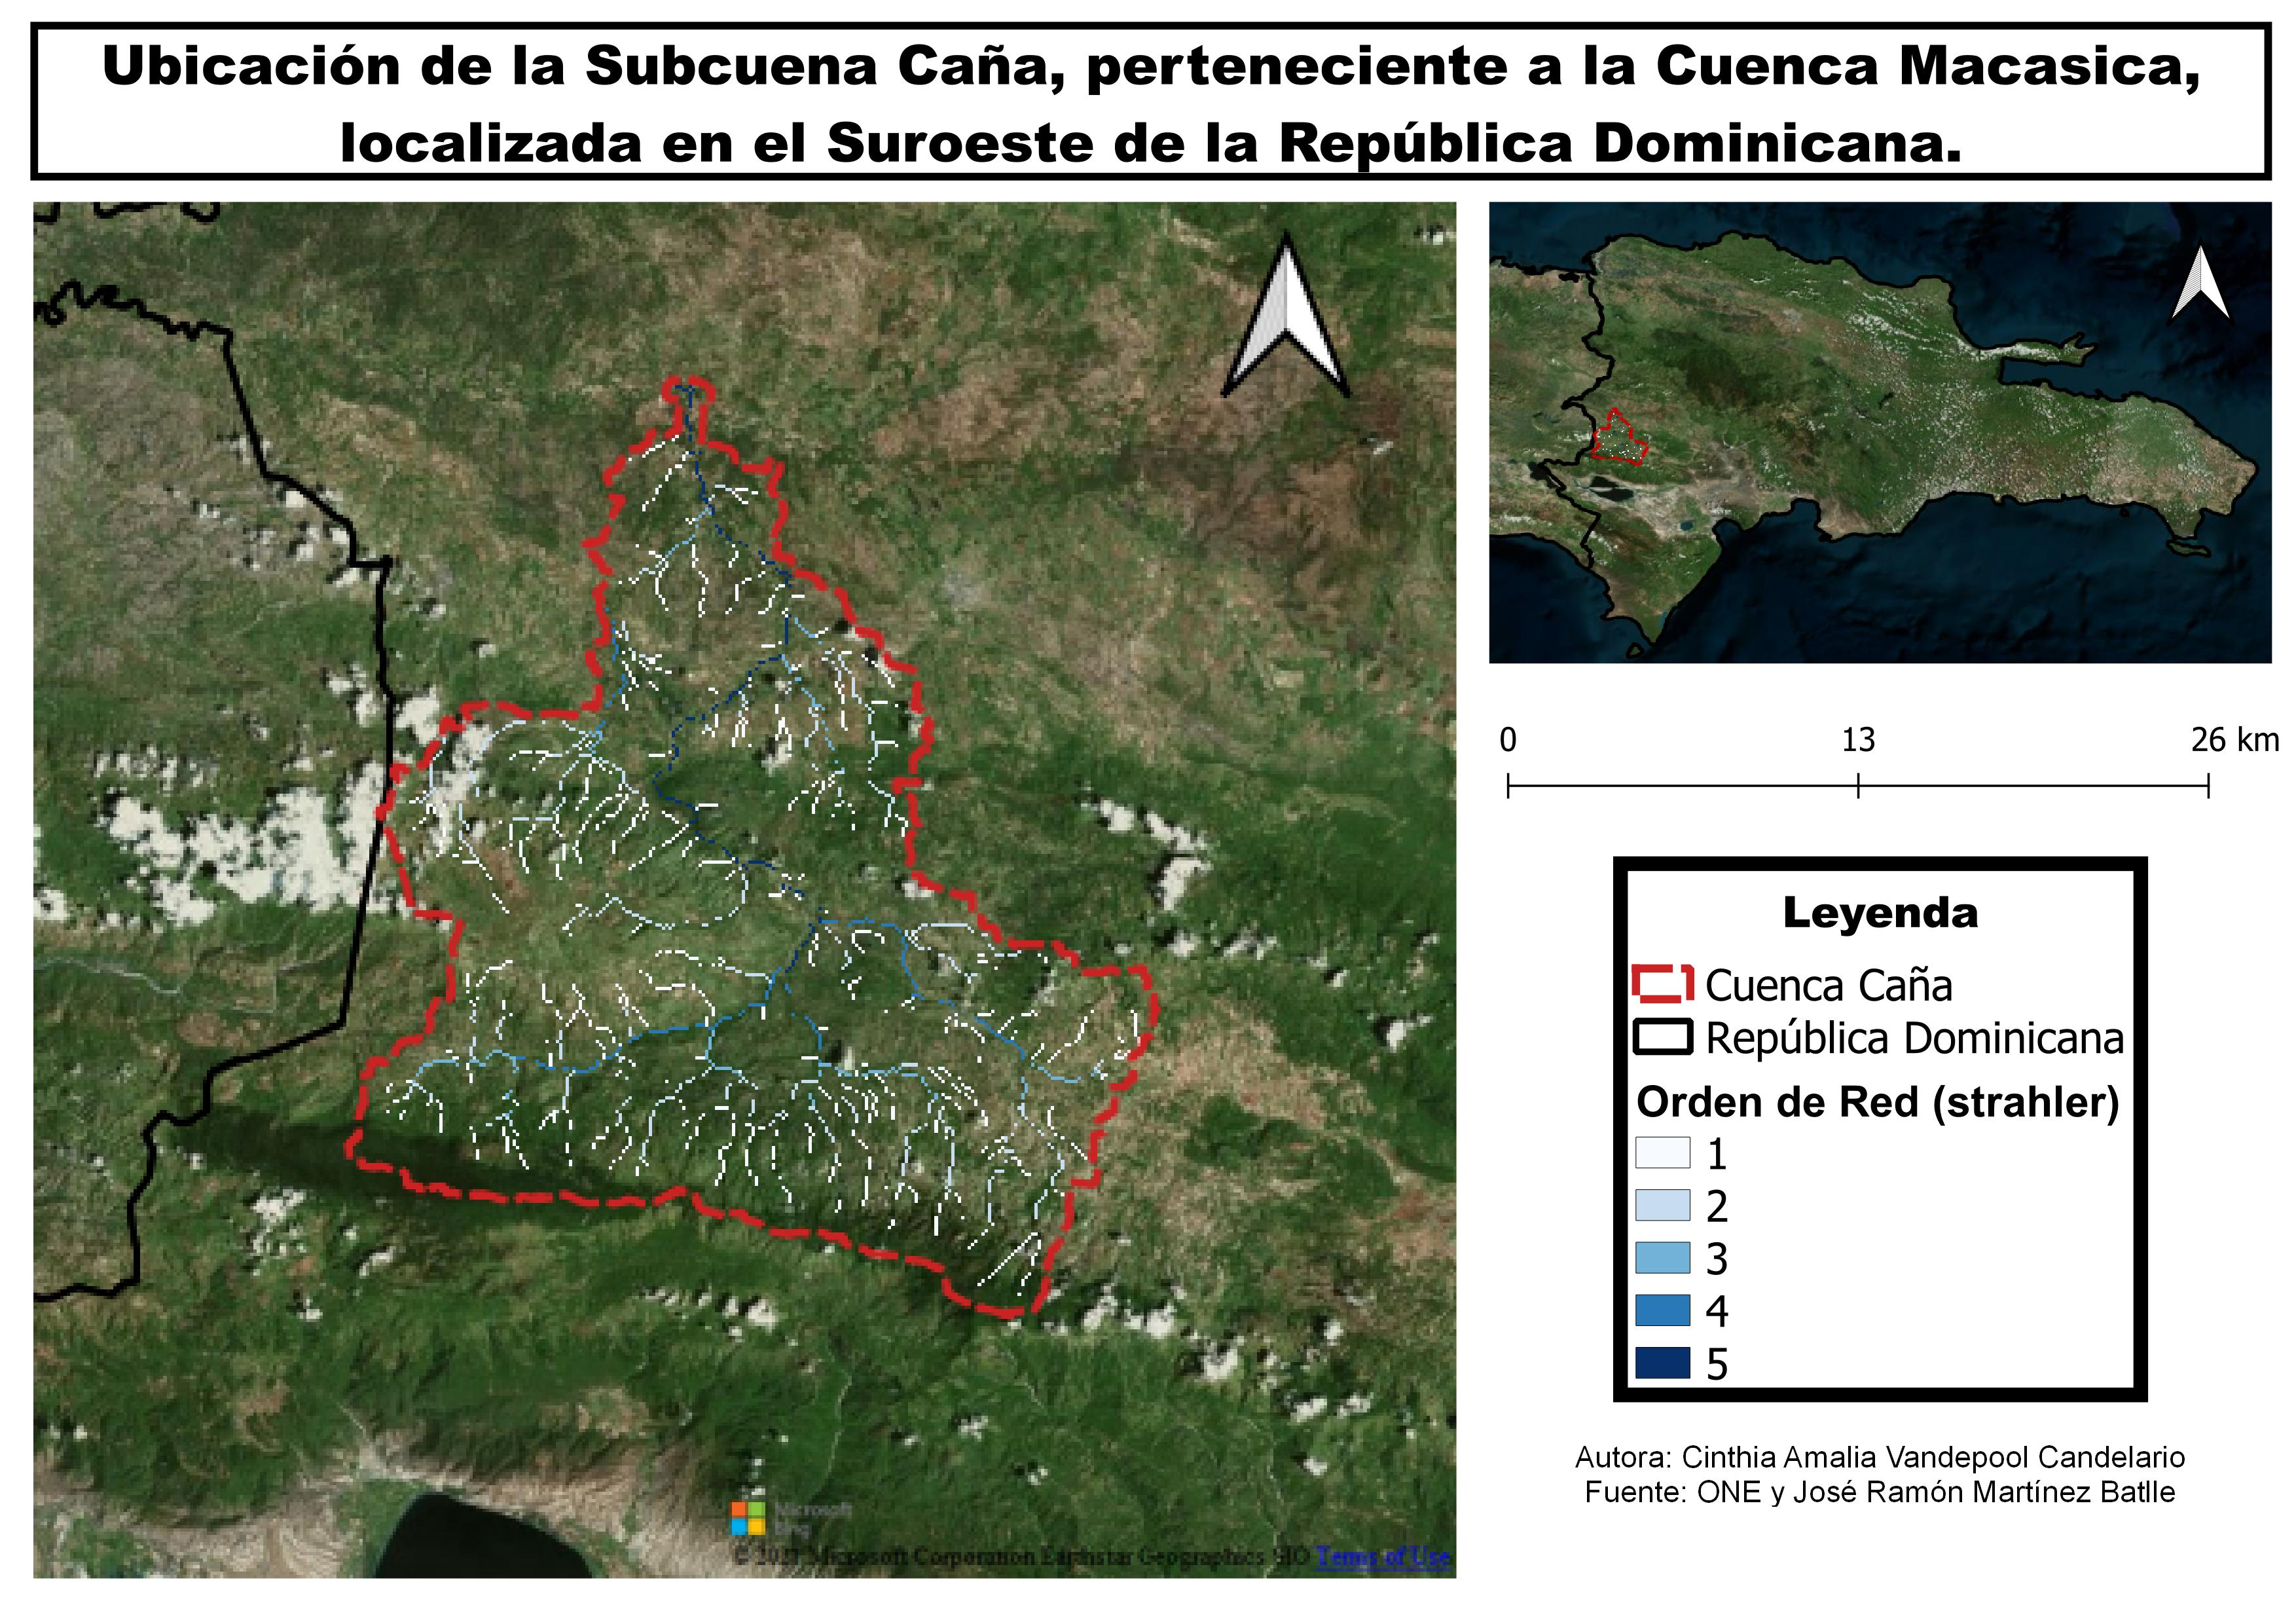
\includegraphics[width=0.75000\textwidth]{mapa_de_subcuenca_cana.jpg}
\caption{Ubicación Microcuenca del Rio Caña}
\end{figure}

De acuerdo al mapa Zonas de Vida (OEA, 1967), la mayor superficie de la
cuenca lo ocupa el Bosque humedo subtropical, se caracteriza por
presentar topografía que varía desde plana hasta accidentada con un
patrón de lluvia que varía de 1000 mm. a 2000 mm.. Según la ubicación de
las áreas, la biotemperatura media anual es de 23ºC a 24ºC con una
evapotranspiración potencial estimada en promedio de 20\% menor que la
precipitación media total anual. El Bosque muy húmedo Montano Bajo es la
segunda en extensión, se caracteriza por la presencia de escarchas
temporales, precipitaciones que alcanzar cantidades mayores a los 2,000
mm. totales anuales con una evapotranspiración potencial estimada en
promedio de 55\% menor que la precipitación media total anual, su
topografía generalmente accidentada con elevaciones que van desde los
850 hasta los 2,100 metros y en menor proporcion lo ocupa el bosque
humedo montano bajo Ministerio de Medio ambiente y Recursos naturales
(2016).

La mayor parte de la cuenca discurre sobre la vertiente Norted del
sistema geomorfologico de la Sierra de Neiba y en menor proporción sobre
el Valle de San juan, siendo la geología conformada, en mayor
proporción, por Caliza tipo Neiba, Marga con calcarenita tipo
sombrerito, Marga con intercalaciones de bancos de caliza arenosa,
arenisca, marga arenosa, conglomerados, conglomerados poligenico, molasa
marina y continental y arena; y en menor proporción está conformada por
caliza en bancos de espesores variables con nodulos e intercalaciones de
pedernal de color blanco-crema, depositos fluviales, depositos
cuaternarios indiferenciados, Basaltos, Tobas, Aglormerados y Rocas
Volcánicas Submarinas Ministerio de Medio ambiente y Recursos naturales
(2016).

\begin{figure}
\centering
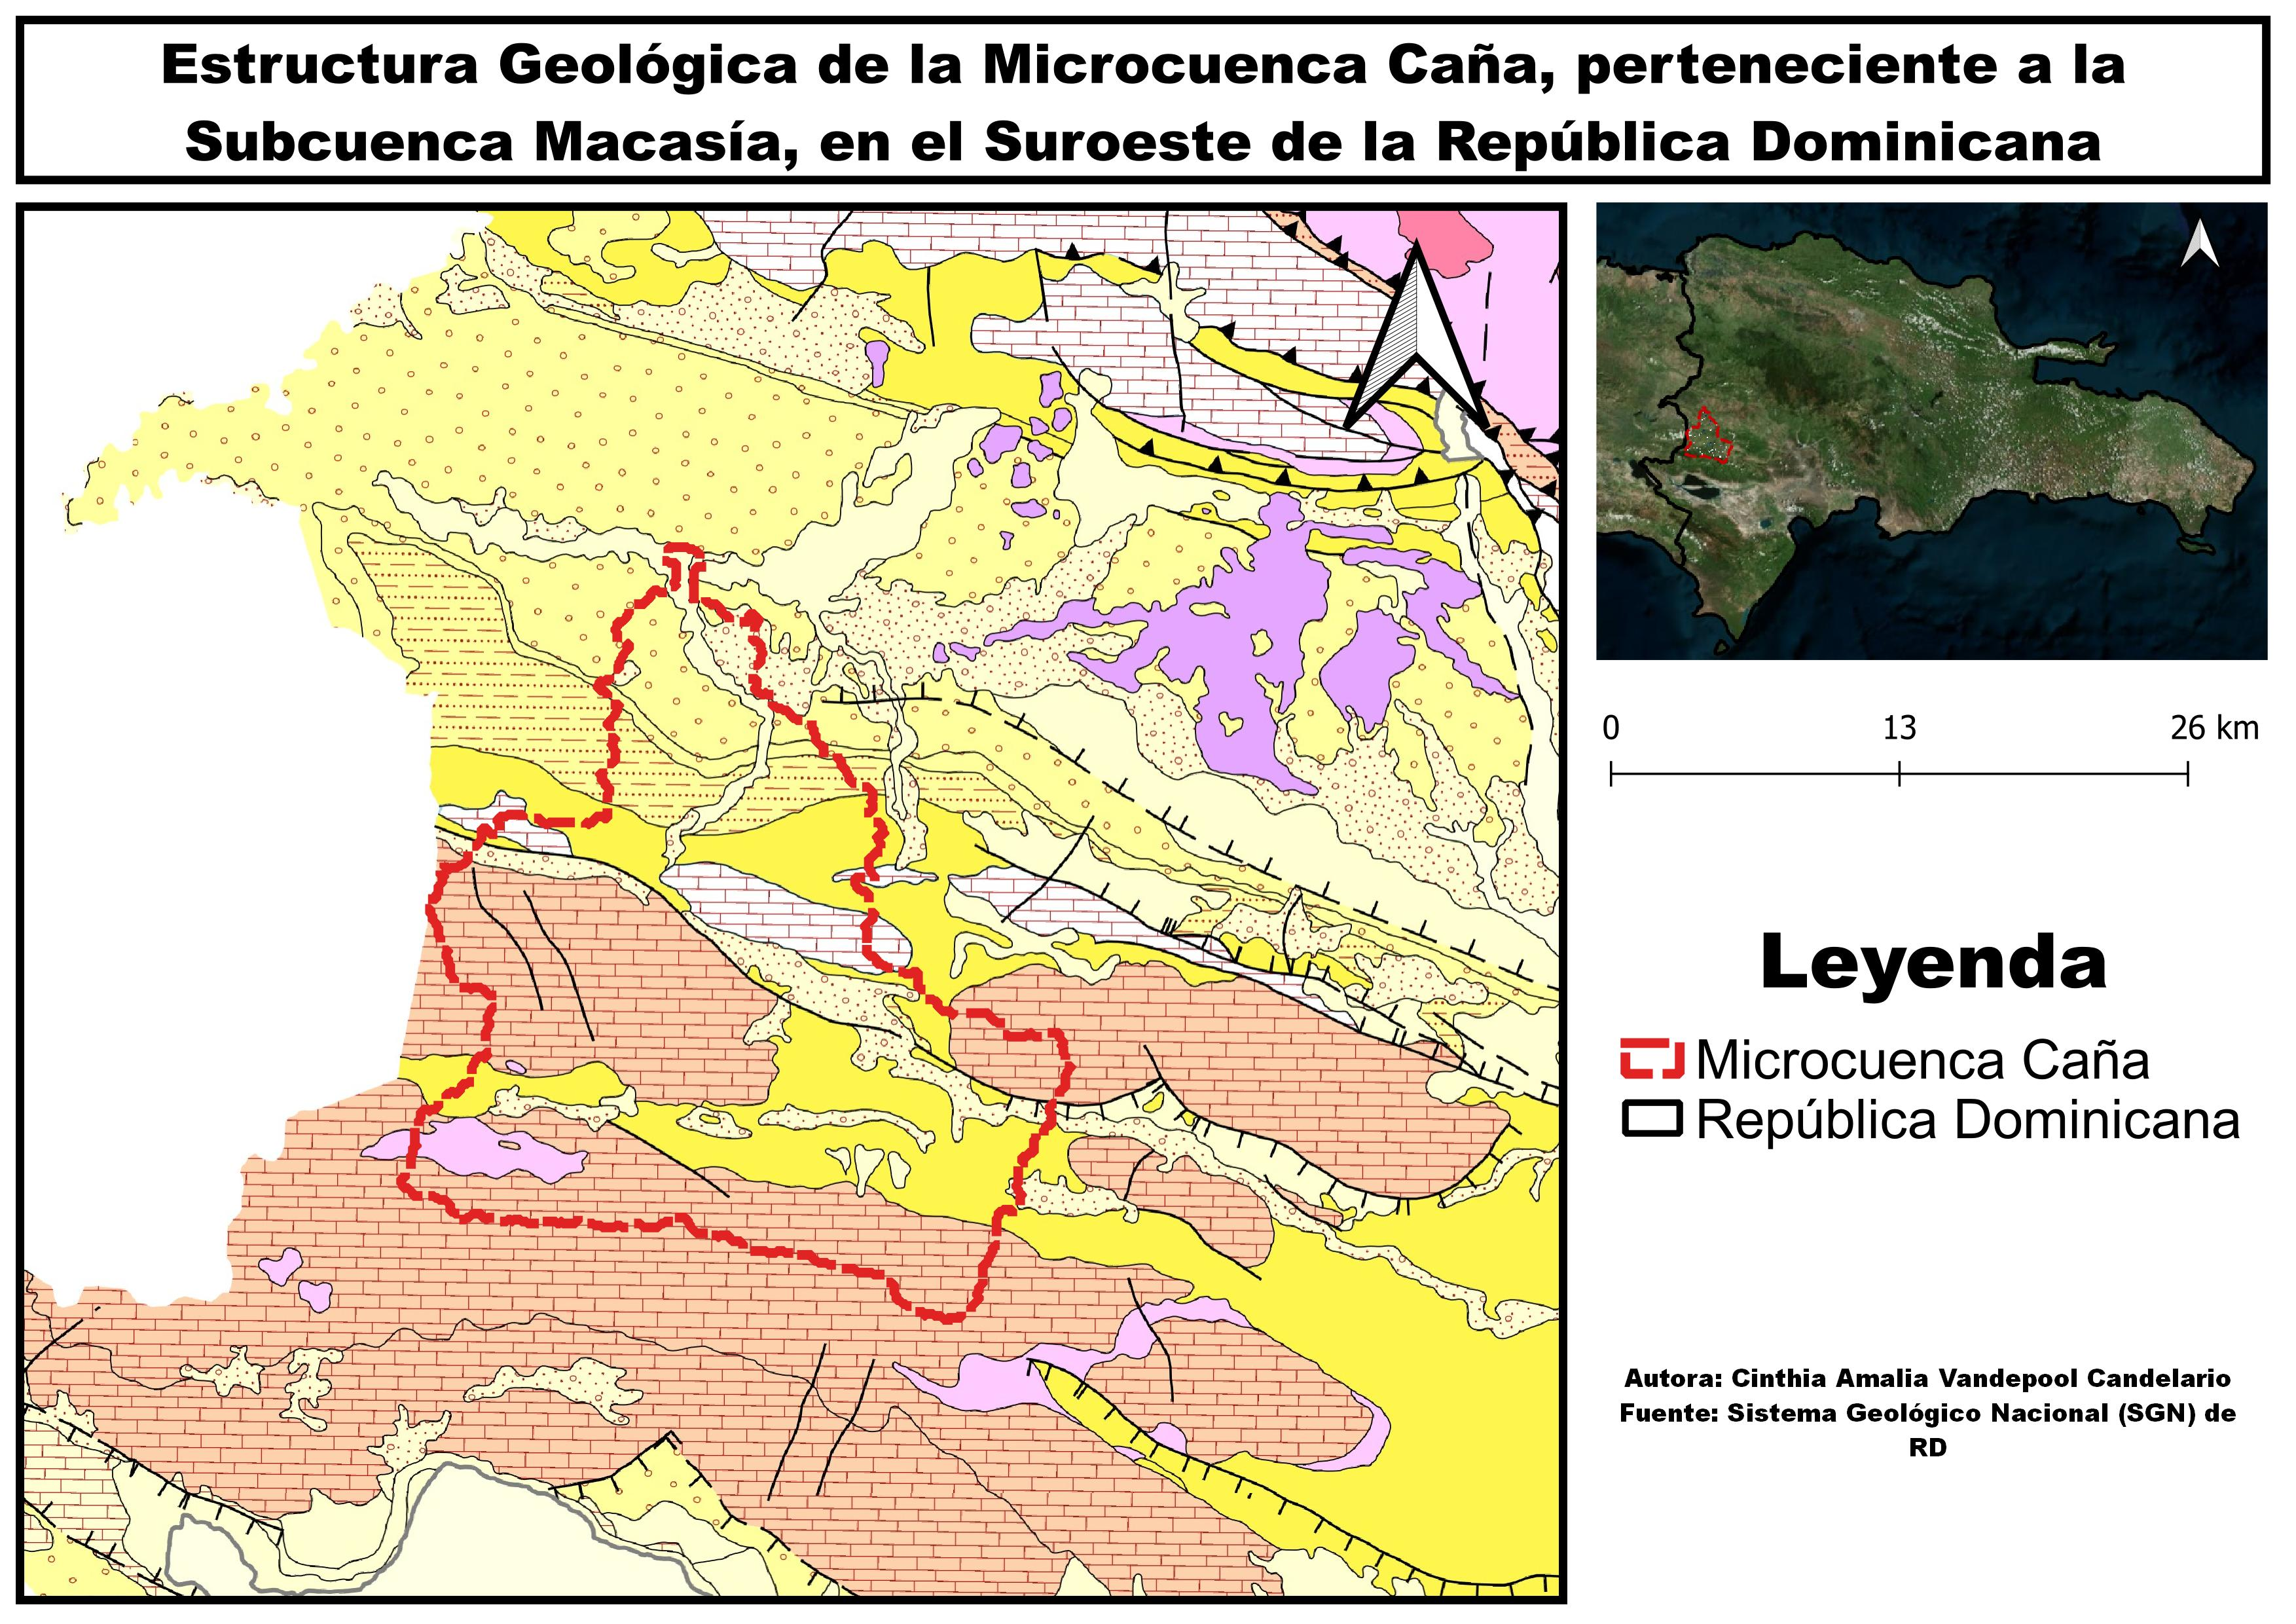
\includegraphics[width=0.75000\textwidth]{mapa_geologico_cuenca_cana.jpg}
\caption{Estructura Geológica de la Microcuenca Caña}
\end{figure}

\subsection{Metodología}\label{metodologuxeda-1}

Para la elaboración de esta investigación se emplearon métodos de
analisis morfometrico a partir de un DEM de la cuenca de interes,
inicialmente cargué una serie de paquetes de Grass en R adecuando el
entorno para ejectar los códigos necesarios.

En primer lugar, se importó a R, como SpatialGridDataFrame, un DEM
alojado en la base de datos de GRASS GIS, se estableció su ruta y
conviertiéndolo a su vez en un objeto raster por medio del paquete
raster de R; partiendo del complemento \emph{r.watershed} (el cual
generá un conjunto de mapas que indican: \emph{la acumulación de flujo,
la dirección del drenaje, la ubicación de los arroyos y las cuencas
hidrográficas} (GRASS Development Team (2003g))) y del modelo digital de
elevaciones (DEM) se generaron diversas capas calculando así los
parámetros hidrográficos de la cuenca del rio caña y sus redes de
drenaje, además, seguido a esto se importó un conjunto de capas ráster
de GRASS GIS a R, como el mapa de red de drenaje y el mapa de cuencas
visualizandolas por medio de \emph{leaflet}.

Utilizando el complemento de GRASS GIS \emph{r.water.outlet} (GRASS
Development Team (2003f)) y apoyandose en los paquetes \emph{mapview}
(Tim Appelhans and others (2020)) y \emph{leaflet} se extrajó la cuenca
de drenaje a partir de un mapa de dirección de flujos con un umbral de
acumulación de \emph{80 celdas} y las coordenadas de la desembocadura de
la cuenca cana (-71.62524,18.94026).

Posteriormente se estableció una máscara usando el límite de la cuenca
caña para luego realizar la extracción partir del DEM de la red de
drenaje utilizando el complemento de GRASS GIS \emph{r.stream.extract}
(GRASS Development Team (2003d)) desde R. Tras esto, se utilizó el
complemento \emph{r.stream}(GRASS Development Team (2003e)) para generar
un mapa de dirección de flujo, \emph{r.stream.order} (GRASS Development
Team (2003b)) para un mapa de orden de red según varios métodos, entre
ellos el método de Strahler y de Horton, a partir de
\emph{r.stream.basins} (GRASS Development Team (2003c)) un mapa de
cuencas según órdenes de red y apoyandose del complemento
\emph{r.stream.stats}(GRASS Development Team (2003a)) se generó las
estadísticas de red resumidas por órdenes, incluyendo la razón de
bifurcación.

\section{Resultados}\label{resultados}

A partir de los codigos ejectudos determinamos que la microcuenca del
rio caña posee una superficie de 525 km\textsuperscript{2} con un
perimetro de 139 km, presentando una forma similiar a la de un triagulo,
presenta mayor extension en el Sur reduciendo su extension asi el Norte.

\begin{figure}
\centering
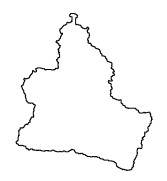
\includegraphics[width=0.30000\textwidth]{area_cana.jpg}
\caption{Área de la microcuenca}
\end{figure}

Esta microcuenca posee una elevacion maxima de 2,231 metros sobre el
nivel del mar, una elevacion minima de 330 metros sobre el nivel del mar
y una elevacion media de 958 metros. Ademas presenta una pendidente de
10.56.

\begin{figure}
\centering
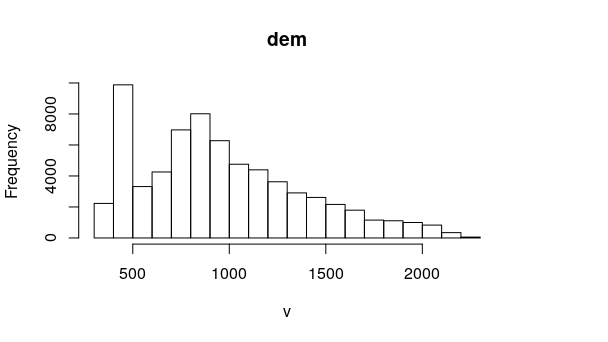
\includegraphics[width=0.50000\textwidth]{pendiente_cana.png}
\caption{Pendiente}
\end{figure}

\section{Discusión}\label{discusiuxf3n}

\section{Agradecimientos}\label{agradecimientos}

\section{Información de soporte}\label{informaciuxf3n-de-soporte}

\ldots

\section{\texorpdfstring{\emph{Script}
reproducible}{Script reproducible}}\label{script-reproducible}

\ldots

\section*{Referencias}\label{referencias}
\addcontentsline{toc}{section}{Referencias}

\hypertarget{refs}{}
\hypertarget{ref-burgos2014modelos}{}
Burgos, V. H., \& Salcedo, A. P. (2014). Modelos digitales de elevación:
Tendencias, correcciones hidrológicas y nuevas fuentes de información.
\emph{Encuentro de Investigadores En Formación En Recursos Hídricos (2,
2014, Ezeiza, Buenos Aires, Argentina). Disponible En: Http://Www. Ina.
Gov. Ar/Ifrh-2014/Eje1/1.11. Pdf. Consultado}, \emph{1}(10), 2015.

\hypertarget{ref-GutierrezElorza}{}
Elorza, M. G. (2008). Geomorfologia fluvia i. In \emph{Geomorfologia}
(pp. 279--283). Pearson Educacion.

\hypertarget{ref-addonrstreamstats}{}
GRASS Development Team. (2003a). Calculates horton's statistics for
strahler and horton ordered networks created with r.stream.order.
Retrieved April 12, 2021, from
\url{https://grass.osgeo.org/grass78/manuals/addons/r.stream.stats.html}

\hypertarget{ref-addonrstreamorder}{}
GRASS Development Team. (2003b). Calculates strahler's and more streams
hierarchy. Retrieved April 12, 2021, from
\url{https://grass.osgeo.org/grass78/manuals/addons/r.stream.order.html}

\hypertarget{ref-addonrstreambasins}{}
GRASS Development Team. (2003c). Delineates basins according stream
network. Retrieved April 12, 2021, from
\url{https://grass.osgeo.org/grass78/manuals/addons/r.stream.basins.html}

\hypertarget{ref-addonrstreamextract}{}
GRASS Development Team. (2003d). Performs stream network extraction.
Retrieved April 12, 2021, from
\url{https://grass.osgeo.org/grass78/manuals/r.stream.extract.html}

\hypertarget{ref-addonrstream}{}
GRASS Development Team. (2003e). R.stream.* modules. Retrieved April 12,
2021, from \url{https://grasswiki.osgeo.org/wiki/R.stream.*_modules}

\hypertarget{ref-addonrwateroutlet}{}
GRASS Development Team. (2003f). R.water.outlet - creates watershed
basins from a drainage direction map. Retrieved April 2, 2021, from
\url{https://grass.osgeo.org/grass78/manuals/r.water.outlet.html}

\hypertarget{ref-addonrwater}{}
GRASS Development Team. (2003g). R.watershed - calculates hydrological
parameters and rusle factors. Retrieved April 2, 2021, from
\url{https://grass.osgeo.org/grass76/manuals/r.watershed.html}

\hypertarget{ref-ibanez2011morfologia}{}
Ibañez Asensio, S., Moreno Ramón, H., \& Gisbert Blanquer, J. M. (2011).
\emph{Morfología de las cuencas hidrológicas}.

\hypertarget{ref-lux2016conceptos}{}
Lux Cardona, B. (2016). \emph{Conceptos básicos de morfometría de
cuencas hidrográficas}.

\hypertarget{ref-MedioAmbiente}{}
Ministerio de Medio ambiente y Recursos naturales. (2016). Macasía.
Retrieved April 28, 2021, from
\url{https://ambiente.gob.do/cuencas-hidrograficas/macasia/}

\hypertarget{ref-mapview}{}
Tim Appelhans and others. (2020). Mapview: Interactive viewing of
spatial data in r. Retrieved April 12, 2021, from
\url{https://cran.r-project.org/web/packages/mapview/index.html}




\newpage
\singlespacing 
\end{document}
